\documentclass[a4j,dvipdfmx]{jarticle}
%----------------------------------------------------------------------
\usepackage{graphicx}
%\usepackage{amsmath}
%\usepackage{amssymb}
%\usepackage{bm}
%\usepackage{fancybox}
\usepackage{fancyhdr}
\usepackage{lastpage}
%\usepackage{color}
\usepackage{multicol}
\usepackage{listings,jlisting}
\usepackage{ascmac}
%----------------------------------------------------------------------
%\setlength{\topmargin}{-0.5in}
%\addtolength{\headheight}{1cm}
%%\setlength{\headsep}{0mm}
%\setlength{\oddsidemargin}{-0.5in}
%%\setlength{\evensidemargin}{-0.5in}
%\addtolength{\textwidth}{1.5in}
%\addtolength{\textheight}{1in}
%----------------------------------------------------------------------
%\setlength{\columnsep}{2zw}
%\setlength{\columnseprule}{0.4pt}
%----------------------------------------------------------------------
\pagestyle{fancy}
\lhead{2016/05/17}
\rhead{配布資料(\thepage / \pageref{LastPage})}
\cfoot{}
\chead{\textgt{システムプログラミング2 第11回}}
%----------------------------------------------------------------------
\begin{document}
\def\lstlistingname{リスト}
\lstset{language=C,
  numbers=left,
  basicstyle={\small\ttfamily},
  columns=[l]{fullflexible},
  keepspaces=true,
  frame=shadowbox,
  commentstyle=\slshape
}
%----------------------------------------------------------------------

%\begin{figure}[hbtp]
%\begin{center}
%\includegraphics[height=2.5cm]{state.pdf}
%\caption{単語の長さをカウントするアルゴリズム}
%\end{center}
%\end{figure}

今回は、環境変数について学ぶ。
環境変数はシェルが管理する変数である。
変数とはいえC言語の変数とは全く別の仕組みである。
プログラムは実行時に環境変数の値を調べることができる。

\begin{enumerate}
\item 環境変数の例

MacやUNIX(Linux,FreeBSD)でよく使用される環境変数の「名前」と「値」の例を示す。
\begin{lstlisting}[numbers=none]
SHELL=/bin/bash                 # 使用中のシェル
TERM=xterm-256color             # 使用中のターミナルエミュレータ
USER=sigemura                   # 現在のユーザ
PATH=:/usr/bin:/bin:/usr...     # シェルがコマンドを探すディレクトリ一覧
PWD=/Users/sigemura             # カレントディレクトリのパス
HOME=/Users/sigemura            # ユーザのホームディレクトリ
LANG=ja_JP.UTF-8                # ユーザが使用したい言語(ja_JP.UTF-8(日本語))
LC_TIME=C                       # ユーザが日時の表示に使用したい言語(C言語標準)
TZ=Japan                        # どの地域の時刻を使用するか(日本)
CLICOLOR=1                      # ls コマンド等がカラー出力する(yes)
\end{lstlisting}

\item 環境変数を変更した例

例えば\verb/LC_TIME/環境変数は日時の表示に使用する言語を決める。
また、\verb/TZ/環境変数はどの地域の時刻を表示するかを決める。
\verb/date/コマンド(現在時刻表示)、\verb/cal/コマンド(カレンダー表示)、
\verb/ls/コマンド(ファイルの最終変更時刻表示)等がこれらの環境変数の値により
日時の表示を変化させる。
\begin{lstlisting}[numbers=none]
$ printenv LC_TIME              # 環境変数 LC_TIME の値を確認する
C                               # C言語標準(米国英語表記)を使用する
$ date
Sun Jun 26 11:04:27 JST 2016    # 英語表示で日本時間
$ ls -l
-rw-r--r--  1 sigemura  staff    319 Jun 26 10:30 Makefile
$ LC_TIME=ja_JP.UTF-8           # LC_TIME に日本語を表す値をセットして試す
$ date
2016年 6月26日 日曜日 11時03分21秒 JST
$ ls -l
rw-r--r--  1 sigemura  staff    319  6 26 10:30 Makefile
$ export TZ=Cuba                # TZ 環境変数を作ってキューバを示す値をセット
$ date
2016年 6月25日 土曜日 22時03分26秒 JST      # 日本語表示でキューバ時間
$
\end{lstlisting}
このようにプログラムの振る舞いを環境変数でコントロールすることができる。

\item 環境変数は誰が決めるか

\begin{enumerate}
\item システム管理者

システム管理者はユーザがログインした時の初期状態を決める。
UNIXやMacでは、\verb;/etc/profile;ファイル等に書かれたスクリプトが
全ユーザのシェル起動時に実行される。
システム管理者は全ユーザに共通の初期化処理をここに書いておく。

\item ユーザの設定ファイル

ユーザは自分のホームディレクトリの\verb;.bash_profile;ファイルに
自分専用の初期化処理を書くことができる。
ここに、「環境変数の操作」で説明するコマンドで処理を書いておく。
次は\verb;.bash_profile;ファイルの例である。

\begin{lstlisting}[numbers=none]
PATH="/usr/local/bin:$PATH:$HOME/bin:."
export LC_TIME=C
export CLICOLOR=1
\end{lstlisting}

\item ユーザによるコマンド操作

シェルのコマンド操作で環境変数を操作することができる。
但し、影響範囲は操作したウインドのシェルのみである。
次回ログイン時には操作結果の影響は残らない。

\end{enumerate}

\item 環境変数の操作

シェルのコマンド操作で環境変数を操作する。
\begin{enumerate}
\item 環境変数の表示

\begin{lstlisting}[numbers=none]
$ printenv             # 全ての環境変数の名前と値を表示する
$ printenv 名前        # 名前の環境変数の値だけを表示する

実行例
$ printenv
SHELL=/bin/bash
TERM=xterm-256color
USER=sigemura
...
$ printenv SHELL
/bin/bash
$
\end{lstlisting}

\item 環境変数の操作

\begin{enumerate}
\item 新規作成(その1)

UNIXの標準シェル(sh)では次の2ステップで環境変数を作る。

\begin{lstlisting}[numbers=none]
$ 変数名=値             # 一旦、シェル変数として作る
$ export 変数名         # シェル変数を環境変数に変更する

実行例
$ printenv MYNAME       # MYNAME環境変数を確認 => 存在しない(何も表示されない)
$ MYNAME=sigemura
$ export MYNAME
$ printenv MYNAME       # MYNAME環境変数を確認 => 値が "sigemura" だとわかる
sigemura
$
\end{lstlisting}

\item 新規作成(その2)

MacやLinuxで使用されるシェル(bash)では、
次のように1行の操作で環境変数を作ることができる。

\begin{lstlisting}[numbers=none]
$ export 変数名=値

実行例
$ printenv MYNAME       # MYNAME環境変数を確認 => 存在しない(何も表示されない)
$ export MYNAME=sigemura
$ printenv MYNAME       # MYNAME環境変数を確認 => 値が "sigemura" だとわかる
sigemura
$
\end{lstlisting}

\item 値の変更

既に存在する環境変数の値を変更する操作は次の通り。
変数名を間違った場合、
間違った名前で新しいシェル変数が作成されエラーにならないので注意が必要である。

\begin{lstlisting}[numbers=none]
$ 変数名=値

実行例
$ MYNAME=yosinaga        # MYNAME環境変数の値を変更
$ printenv MYNAME        # MYNAME環境変数の値が変更されている
yosinaga
$
\end{lstlisting}

\item 値の参照

「\verb/$変数名/」と書くことにより
環境変数やシェル変数の値をコマンド入力時に参照できる。
例えば、すでにある\verb/PATH/環境変数の値に新規ディレクトリを追加する例を示す。
\begin{lstlisting}[numbers=none]
$ printenv PATH                    # 初期状態を確認する
/usr/local/bin:/bin:/usr/bin
$ PATH=$PATH:.                     # カレントディレクトリを追加する
$ printenv PATH
/usr/local/bin:/bin:/usr/bin:.
$ PATH=$PATH:$HOME/bin             # ホームのbinディレクトリを追加する
$ printenv PATH
/usr/local/bin:/bin:/usr/bin:./User/sigemura/bin
$
\end{lstlisting}

\item 変数の削除

環境変数、シェル変数のどちらも次の操作で削除できる。
存在しない変数を\verb/unset/してもエラーにならない。
変数名を間違ってもエラーにならないので注意が必要である。

\begin{lstlisting}[numbers=none]
$ unset 変数名

実行例
$ unset MYNAME
$ printenv MYNAME       # MYNAME環境変数を確認 => 存在しない(何も表示されない)
$
\end{lstlisting}

\item 値を一時的に変更

変数の値を一時的(今回のコマンド実行の期間だけ)に
変更してコマンド(プログラム)を実行する。

\begin{lstlisting}[numbers=none]
$ env 変数名=値 ...  コマンド

実行例
$ date
Sun Jul  3 08:35:42 JST 2016
$ env LC_TIME=ja_JP.UTF-8 TZ=Cuba date    # 日本語表示、キューバ時間でdate実行
2016年 7月 2日 土曜日 19時36分01秒 CDT
$ date
Sun Jul  3 08:36:05 JST 2016
$
\end{lstlisting}

\end{enumerate}

\end{enumerate}

\item 環境変数の仕組み

図\ref{fig1}に環境変数の仕組みを示す。

\begin{figure}[hbtp]
  \begin{center} %センタリングする
    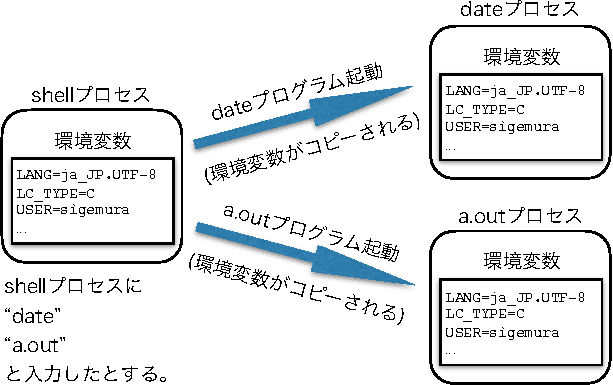
\includegraphics[scale=0.8]{fig1-crop.pdf}
    \caption{プログラム起動時の環境変数コピー}
    \label{fig1}
  \end{center}
\end{figure}

シェルプロセス(shellプロセス)は
環境変数を自プロセスのメモリ空間で記憶・管理している。
上記の「環境変数の操作」で紹介したコマンド等は、
シェルのメモリ空間の環境変数・シェル変数を操作するものである。
このようにシェル自身が処理するコマンドを{\bf 内部コマンド}と呼ぶ。

シェルは入力されたコマンドが内部コマンド以外({\bf 外部コマンド})なら、
コマンド名と同じ名前のプログラムを探し子プロセスとして起動する。
この時シェルは、
自身の環境変数を子プロセスにコピーするようにOSカーネルに依頼する。
OSカーネルは子プロセスのメモリ空間のどこか(例えばスタックの底)に
環境変数をコピーする。
子プロセスはメモリ空間内の環境変数のコピーを参照・変更・削除できる。

この仕組みはシェルに限らず全ての{\bf 他のプログラムを起動するプログラム}で
用いられる仕組みである。
実は上記の「環境変数の操作」で紹介した操作方法で
\verb/env/コマンドだけは{\bf 外部コマンド}である。
\verb/env/コマンドは{\bf 他のプログラムを起動するプログラム}として実装できる。

図\ref{fig2}に\verb/env/コマンドの仕組みを示す。
\verb/env/コマンドは自身の環境変数を変更した後、
目的のコマンドを起動する。

\begin{figure}[hbtp]
  \begin{center} %センタリングする
    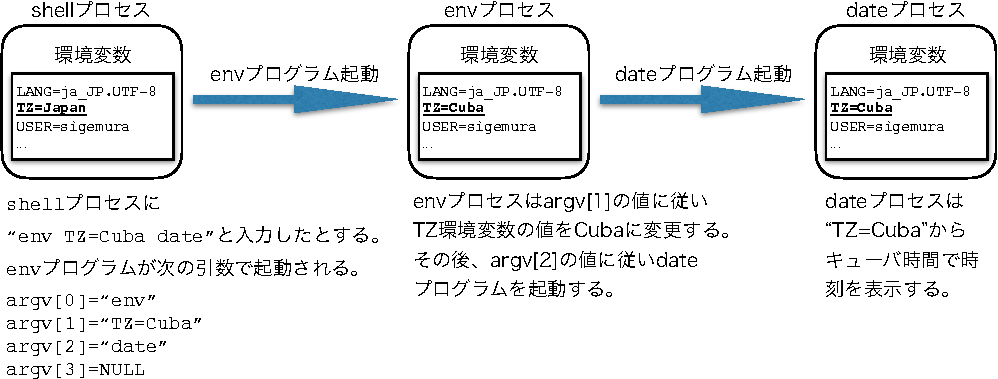
\includegraphics[scale=0.8]{fig2-crop.pdf}
    \caption{env プログラムの仕組み}
    \label{fig2}
  \end{center}
\end{figure}

\item C言語プログラムから環境変数を参照する方法

C言語プログラムから環境変数を参照するために、
以下に紹介する二つの方法が使用できる。

\begin{enumerate}
\item main関数の仮引数やグローバル変数environを使用する方法

C言語の\verb/main/関数には実は第3引数が存在した。
\verb/environ/という名前のC言語のグローバル変数が存在する。

\begin{lstlisting}[numbers=none]
extern char **environ;  // どこかで定義されているenviron変数を使用する準備
int main(int argc, char *argv[], char *envp[]) { ...
\end{lstlisting}

図\ref{fig3}にプロセスのメモリ空間にコピーされた環境変数のデータ構造を示す。

\begin{figure}[tbph]
  \begin{center} %センタリングする
    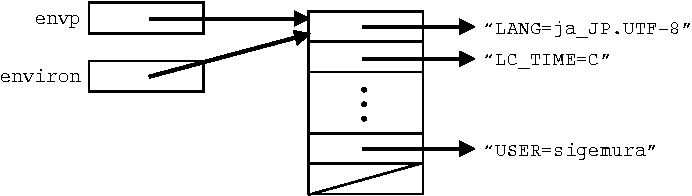
\includegraphics[scale=0.8]{fig3-crop.pdf}
    \caption{環境変数のデータ構造}
    \label{fig3}
  \end{center}
\end{figure}

例えば全ての環境変数を表示するCプログラムは次のように書くことができる。

\lstinputlisting[numbers=none]{envtest1.c}

\item getenv関数を使用する方法

C言語標準ライブラリの\verb/getenv/関数は次のような書式の関数である。

\begin{lstlisting}[numbers=none]
書式
#include <stdlib.h>
char *getenv(char *name);
\end{lstlisting}

\verb/name/には環境変数名を渡す。
\verb/getenv/は環境変数の値を示す文字列を指すポインタを返す。
\verb/name/の環境変数が見つからない場合は\verb/NULL/ポインタを返す。
次のCプログラムは\verb/LANG/環境変数の値を表示するものである。

\lstinputlisting[numbers=none]{envtest2.c}

\end{enumerate}

\item C言語プログラムから環境変数を操作する方法

自プロセスのメモリ空間に置かれた環境変数のコピーを操作する
三つのC言語標準ライブラリ関数を紹介する。

\begin{enumerate}
\item setenv関数

環境変数を新規に作成したり、値を上書きしたりする関数である。
\verb/overwrite/が\verb/0/の時は新規作成専用になる。

\begin{lstlisting}[numbers=none]
書式
#include <stdlib.h>
int setenv(char *name, char *val, int overwrite);

使用例
setenv("MYNAME", "sigemura", 1);
\end{lstlisting}

\verb/name/は環境変数の名前、
\verb/val/は環境変数にセットする値である。
\verb/overwrite/は、
\verb/0/の時に上書き禁止、
それ以外の時に上書き許可を意味する。
\verb/setenv/の返す値が\verb/0/は正常、
それ以外はエラーである。

\item putenv関数

環境変数を新規に作成したり、値を上書きしたりする関数である。

\begin{lstlisting}[numbers=none]
書式
#include <stdlib.h>
int putenv(char *string);

使用例
putenv("MYNAME=sigemura");
\end{lstlisting}

\verb/string/は\verb/NAME=VALUE/形式の文字列である
(それ以外の形式の文字列を渡すとエラーになる)。
\verb/putenv/の返す値は\verb/0/が正常、それ以外はエラーである。
\verb/putenv("NAME=VALUE");/は、
\verb/setenv("NAME","VALUE",1);/と同じ操作を行う。

\item unsetenv関数

環境変数を削除する関数である。

\begin{lstlisting}[numbers=none]
書式
#include <stdlib.h>
int unsetenv(char *name);

使用例
unsetenv("MYNAME");
\end{lstlisting}

\verb/name/は環境変数の値である。
\verb/unsetenv/の返す値は\verb/0/が正常、それ以外はエラーである。

\end{enumerate}

\item 宿題

\begin{enumerate}
\item 上記の実行例を試してみる

環境変数を操作するシェルの{\bf 内部コマンド}、{\bf 外部コマンド}を使用してみる。
下の囲み記事を参考に、
\verb/LC_TIME/環境変数や\verb/TZ/環境変数を色々試すと面白い。
例えば、「モスクワ時間、ロシア語表示」で時刻を表示するにはどうしたらよいか?

\item myprintenvプログラム

\verb/printenv/と同様な働きをする\verb/myprintenv/プログラムを作成する。
作成したプログラムを印刷して提出する。

〆切:7月8日(金)

\end{enumerate}

\begin{itembox}[l]{ロケール}
\verb/LANG/環境変数や\verb/LC_TIME/環境変数にセットする値をロケール名と呼ぶ。
ロケール名は\verb/"言語コード_国名コード.エンコーディング"/の組み合わせで
表現される。

言語コードはISO639で定義された2文字コードである(日本語は"ja")。
詳しくは\verb;https://ja.wikipedia.org/wiki/ISO_639-1;等を参照のこと。

国名コードはISO3166で定義された2文字コードである(日本は"JP")。
詳しくは\verb;https://ja.wikipedia.org/wiki/ISO_3166-1;等を参照のこと。

エンコーディングは、使用する文字コードの符号化方式を示す。
エンコーディング方式がターミナルエミュレータの
テキストエンコーディングと一致していないと文字化けを起こす。
使用可能なロケールの一覧は\verb/locale -a/コマンドで表示できる。
\end{itembox}

\begin{itembox}[l]{タイムゾーン}
\verb/TZ/環境変数にタイムゾーンを表す値をセットする。
MacOSやUNIXの内部では時刻は協定世界時(UTC)で管理されている。
時刻を表示する時に現地時間に変換して表示する。

時刻に関係するプログラムは
協定世界時と現地時間の変換方法を\verb/TZ/環境変数から知ることができる。
日本の場合はタイムゾーン名が\verb/JST/、協定世界時との時差が$-9$時間なので、
\verb/TZ=JST-9/となる。

この形式の他に\verb;/usr/share/zoneinfo/;に置いてあるファイル名で
タイムゾーンを指定することもできる。
\verb;/usr/share/zoneinfo/Cuba;ファイルが存在するので
\verb;TZ=Cuba;と指定できる。
\verb;/usr/share/zoneinfo/Asia/Tokyo;ファイルが存在するので
\verb;TZ=Asia/Tokyo;と指定できる。
\end{itembox}

\end{enumerate}
\end{document}
